\documentclass[11pt]{article} 
\usepackage[english]{babel}
\usepackage[utf8]{inputenc}
\usepackage[margin=0.5in]{geometry}
\usepackage{amsmath}
\usepackage{amsthm}
\usepackage{amsfonts}
\usepackage{amssymb}
\usepackage[usenames,dvipsnames]{xcolor}
\usepackage{graphicx}
\usepackage[siunitx]{circuitikz}
\usepackage{tikz}
\usepackage[colorinlistoftodos, color=orange!50]{todonotes}
\usepackage{hyperref}
\usepackage[numbers, square]{natbib}
\usepackage{fancybox}
\usepackage{epsfig}
\usepackage{soul}
\usepackage[framemethod=tikz]{mdframed}
\usepackage[shortlabels]{enumitem}
\usepackage[version=4]{mhchem}
\usepackage{multicol}
\usepackage{forest}
\usepackage{mathtools}
\usepackage{comment}
\usepackage{enumitem}
\usepackage[utf8]{inputenc}
\usepackage[linesnumbered,ruled,vlined]{algorithm2e}
\usepackage{listings}
\usepackage{color}
\usepackage[numbers]{natbib}
\usepackage{subfiles}
\usepackage{tkz-berge}


\newtheorem{prop}{Proposition}[section]
\newtheorem{thm}{Theorem}[section]
\newtheorem{lemma}{Lemma}[section]
\newtheorem{cor}{Corollary}[prop]

\theoremstyle{definition}
\newtheorem{definition}{Definition}

\theoremstyle{definition}
\newtheorem{required}{Problem}

\theoremstyle{definition}
\newtheorem{ex}{Example}


\setlength{\marginparwidth}{3.4cm}
%#########################################################

%To use symbols for footnotes
\renewcommand*{\thefootnote}{\fnsymbol{footnote}}
%To change footnotes back to numbers uncomment the following line
%\renewcommand*{\thefootnote}{\arabic{footnote}}

% Enable this command to adjust line spacing for inline math equations.
% \everymath{\displaystyle}

% _______ _____ _______ _      ______ 
%|__   __|_   _|__   __| |    |  ____|
%   | |    | |    | |  | |    | |__   
%   | |    | |    | |  | |    |  __|  
%   | |   _| |_   | |  | |____| |____ 
%   |_|  |_____|  |_|  |______|______|
%%%%%%%%%%%%%%%%%%%%%%%%%%%%%%%%%%%%%%%

\title{
\normalfont \normalsize 
\textsc{CSCI 3104 Fall 2021 \\ 
Instructors: Profs. Grochow and Waggoner} \\
[10pt] 
\rule{\linewidth}{0.5pt} \\[6pt] 
\huge Problem Set 1 \\
\rule{\linewidth}{2pt}  \\[10pt]
}
%\author{}
\date{}

\begin{document}

\maketitle


%%%%%%%%%%%%%%%%%%%%%%%%%
%%%%%%%%%%%%%%%%%%%%%%%%%%
%%%%%%%%%%FILL IN YOUR NAME%%%%%%%
%%%%%%%%%%AND STUDENT ID%%%%%%%%
%%%%%%%%%%%%%%%%%%%%%%%%%%
\noindent
Due Date \dotfill September 7, 2021 \\
Name \dotfill \textbf{Michael Ghattas} \\
Student ID \dotfill \textbf{109200649} \\
Collaborators \dotfill \textbf{Francesca Tenney}

\tableofcontents

\section{Instructions}
 \begin{itemize}
	\item The solutions \textbf{should be typed}, using proper mathematical notation. We cannot accept hand-written solutions. \href{http://ece.uprm.edu/~caceros/latex/introduction.pdf}{Here's a short intro to \LaTeX.}
	\item You should submit your work through the \textbf{class Canvas page} only. Please submit one PDF file, compiled using this \LaTeX \ template.
	\item You may not need a full page for your solutions; pagebreaks are there to help Gradescope automatically find where each problem is. Even if you do not attempt every problem, please submit this document with no fewer pages than the blank template (or Gradescope has issues with it).

	\item You are welcome and encouraged to collaborate with your classmates, as well as consult outside resources. You must \textbf{cite your sources in this document.} \textbf{Copying from any source is an Honor Code violation. Furthermore, all submissions must be in your own words and reflect your understanding of the material.} If there is any confusion about this policy, it is your responsibility to clarify before the due date. 

	\item Posting to \textbf{any} service including, but not limited to Chegg, Reddit, StackExchange, etc., for help on an assignment is a violation of the Honor Code.

	\item You \textbf{must} virtually sign the Honor Code (see Section \ref{HonorCode}). Failure to do so will result in your assignment not being graded.
\end{itemize}


\section{Honor Code (Make Sure to Virtually Sign)} \label{HonorCode}

\begin{required}
\begin{itemize}
\item My submission is in my own words and reflects my understanding of the material.
\item Any collaborations and external sources have been clearly cited in this document.
\item I have not posted to external services including, but not limited to Chegg, Reddit, StackExchange, etc.
\item I have neither copied nor provided others solutions they can copy.
\end{itemize}

%\noindent In the specified region below, clearly indicate that you have upheld the Honor Code. Then type your name. 
\end{required}

\begin{proof}[Answer:]
\item \textbf{I agree to the above, Michael Ghattas.}
%% Typing "I agree to the above," followed by your name is sufficient.
\end{proof}


\newpage
\section{Standard 1- Proof by Induction}

\subsection{Problem \ref{Induction1}}
\begin{required} \label{Induction1}
A student is trying to prove by induction that $2^{n} < n!$ for $n \geq 4$. 

\begin{proof}[Student's Proof]
The proof is by induction on $n \geq 4$. 
\begin{itemize}
\item \textbf{Base Case:} When $n = 4$, we have that:
\begin{align*}
2^{4} &= 16 \\
&\leq 24 \\
&= 4!
\end{align*}

\item \textbf{Inductive Hypothesis:} Now suppose that for all $k \geq 4$ we have that $2^{k} < k!$. 

\item \textbf{Inductive Step:} We now consider the $k+1$ case. We have that $2^{k+1} < (k+1)!$. It follows that $2^{k} < k!$. The result follows by induction.
\end{itemize}
\end{proof}

There are two errors in this proof. 
\begin{enumerate}[label=(\alph*)]
\item The Inductive Hypothesis is not correct. Write an explanation to the student explaining why their Inductive Hypothesis is not correct. [\textbf{Note:} You are being asked to explain why the Inductive Hypothesis is wrong, and \textbf{not} to rewrite a corrected Inductive Hypothesis.]


\begin{proof}[Answer:]
\item \textbf{The in the Inductive Hypothesis is claiming $[2^{k} < (k)!]$ holds $\forall k\ (k \geq 4)$ such that $k\in\mathbb{N}$, instead of stating that $\forall k\ (k > 4)$, $[2^{k-1} < (k-1)!]$ where $k\in\mathbb{N}$ holds true, in order to prove the original assumption in the Inductive Step.}
%Your answer goes here
\end{proof}


\vskip 15pt
\item The Inductive Step is not correct. Write an explanation to the student explaining why their Inductive Step is not correct. [\textbf{Note:} You are being asked to explain why the Inductive Step is wrong, and \textbf{not} to rewrite a corrected Inductive Step.]

\begin{proof}[Answer:]
\item \textbf{The first error in the Inductive Step is they should have stated IF  $[2k < k!]$ is true, THEN it should follow that 
$[2^{k-1} < (k - 1)!]$ is also true $\forall k\ (k > 4)$, and then provide the proof of the claim through a step-by step mathematical justification. Additionally, there should have been a conclusion clearly stating the result and its logical link to the Inductive Hypothesis and claim in the Inductive Step.}
%Your answer goes here
\end{proof}
\end{enumerate}
\end{required}





\newpage
\subsection{Problem \ref{Induction2}} 
\begin{required} \label{Induction2}
Consider the recurrence relation, defined as follows:
\[
T_{n} = \begin{cases} 1 & : n = 0, \\
11 & : n = 1, \\
T_{n-1} + 12T_{n-2} & : n \geq 2.
\end{cases}
\]

\noindent Prove by induction that $T_{n} = (-1) \cdot (-3)^{n} + 2 \cdot (4)^{n}$, for all integers $n \in \mathbb{N}$. [\textbf{Recall:} $\mathbb{N} = \{0, 1, 2, \ldots \}$ is the set of non-negative integers.]
\end{required}

\begin{proof}\textbf{By induction on $n \in \mathbb{N}$}
\begin{itemize}

\item \textbf{Base Case:}
\\ \textbf{When $(n = 0)$,}
\begin{align*}
T_0 &= (-1)*(-3)^0+2*(4)^0 \\
&= (-1)*(1)+2*(1) \\
&= -1+2 \\
&= 1
\end{align*}

\textbf{When $(n = 1)$,}
\begin{align*}
T_1 &= (-1)*(-3)^1+2*(4)^1 \\
&= (-1)*(-3)+2*(4) \\
&= 3+8 \\
&= 11
\end{align*}

\textbf{When $(n = 2)$,}
\begin{align*}
T_2 &= (-1)*(-3)^2+2*(4)^2 \\
&= (-1)*(9)+2*(16) \\
&= -9+32 \\
&= 23 \\
\\
&= T_1+12*T_0 \\
&= 11+12*1 \\
&= 11+12 \\
&= 23
\end{align*}

\textbf{When $(n = 3)$,}
\begin{align*}
T_3 &= (-1)*(-3)^3+2*(4)^3 \\
&= (-1)*(-27)+2*(64) \\
&= 27+128 \\
&= 155 \\
\\
&= T_2+12*T_1 \\
&= 23+12*11 \\
&= 23+132 \\
&= 155
\end{align*}

\textbf{Thus the base cases of $[T_{n} = (-1) \cdot (-3)^{n} + 2 \cdot (4)^{n}]$ for $(n=0,1,2,3)$ hold true.}

\item \textbf{Inductive Hypothesis: Fix $k \geq 0$, and suppose $(0 \leq n \leq k)$ for $[T_{k+1} = T_k + T_{k-1}]$ holds true.}

\item \textbf{Inductive Step: We now consider the $(k+1)$ case. If $[T_{k+1} = T_k + T_{k-1}]$ for $k \in \mathbb{N}$ holds true, then it follows that $T_{k+1} = (-1) \cdot (-3)^{k+1} + 2 \cdot (4)^{k+1}$ also is true. The result follows by induction:}


\begin{align*}
T_{k+1} &= T_k + T_{k-1} \\
&= [(-1)*(-3)^{k}+2*(4)^{k}] + 12*[(-1)*(-3)^{k-1}+2*(4)^{k-1}] \\
&= [(-1)*(-3)^{k}+2*(4)^{k}] + 12*[(-1)*(-3)^{-1}*(-3)^{k}+2*(4)^{-1}*(4)^{k}] \\
&= [(-1)*(-3)^{k}+2*(4)^{k}] + 12*[(-1)*(-1/3)*(-3)^{k}+2*(1/4)*(4)^{k}] \\
&= [(-1)*(-3)^{k}+2*(4)^{k}] + 12*[((1/3)*(-3)^{k}+(2/4)*(4)^{k}] \\
&= [(-1)*(-3)^{k}+2*(4)^{k}] + [(12*((1/3)*(-3)^{k})+(12*(1/2)*(4)^{k})] \\
&= [(-1)*(-3)^{k}+2*(4)^{k}] + [((12/3)*(-3)^{k})+((12/2)*(4)^{k})] \\
&= [(-1)*(-3)^{k}+2*(4)^{k}] + [((4)*(-3)^{k})+((6)*(4)^{k})] \\
&= (-1)*(-3)^{k}+2*(4)^{k}+(4)*(-3)^{k}+(6)*(4)^{k} \\
&= (-1)*(-3)^{k}+(4)*(-3)^{k}+2*(4)^{k}+(6)*(4)^{k} \\
&= 3*(3)^{k}+8*(4)^{k} \\
&= (-1*(-3))*(-3)^{k}+(2*(4))*(4)^{k} \\
&= -1*(-3)^{k+1}+2*(4)^{k+1} 
\end{align*}

\textbf{Conclusion: $T_{n+1}$ holds true as per our induction, thus the argument is true $\forall n\ $$n \in \mathbb{N}$.}
\end{itemize}
%Your proof goes here.
\end{proof}



\newpage
\subsection{Problem \ref{Induction3}}
\begin{required} \label{Induction3}
The complete, balanced 4-ary tree of depth $d$, denoted $\mathcal{T}(d)$, is defined as follows. 
\begin{itemize}
\item $\mathcal{T}(0)$ consists of a single vertex.
\item For $d > 0$, $\mathcal{T}(d)$ is obtained by starting with a single vertex and setting each of its four children to be copies of $\mathcal{T}(d-1)$.
\end{itemize}

\noindent Prove by induction that $\mathcal{T}(d)$ has $4^{d}$ leaf nodes. To help clarify the definition of $\mathcal{T}(d)$, illustrations of $\mathcal{T}(0), \mathcal{T}(1)$, and $\mathcal{T}(2)$ are on the next page. [\textbf{Note:} $\mathcal{T}(d)$ is a tree and \textbf{not} the number of leaves on the tree. Avoid writing $\mathcal{T}(d) = 4^{d}$, as these data types are incomparable: a tree is not a number.]
\end{required}

\begin{proof}\textbf{By induction on $d \in \mathbb{N}$}
\begin{itemize}

\item \textbf{Base Case: \\}
\\ \textbf{When $(d = 0)$, $T(0)$ consists of a single vertex, which is a single leaf node by definition. \\
i.e. $T(0)$ has $[(4^{0})=1]$ leaf node. \\}
\\ \textbf{When $(d = 1)$, $T(1)$ consists of four leaf nodes. \\
i.e. $T(1)$ has $[(4^{1})=4]$ leaf nodes. \\}
\\ \textbf{When $(d = 2)$, $T(1)$ consists of 16 leaf nodes. \\
i.e. $T(1)$ has $[(4^{2})=16]$ leaf nodes. \\}

\textbf{Thus the claim for $(d=0,1,2)$ holds true. \\}

\item \textbf{Inductive Hypothesis: Fix $k \geq 0$, and suppose $(0 \leq d \leq k)$ for tree $T(k)$ consists of $(4^{k})$ leaf nodes.}

\item \textbf{Inductive Step: We now consider Consider $T(k+1)$, which by definition, consists of a root node $(v)$, where each of $(v)'s$ four children are copies of $T(k)$, a complete and balanced tree with each leaf of the $k^{th}$ level has four children. Accordingly, by the inductive hypothesis, $T(k)$ has $(4^{k})$ leaf nodes, where $(v)$ has four children, and $T(k+1)$ has in total:}


\begin{align*}
4*[(4^{k})] &= (4)*(4^{k}) \\
&= 4^{k+1} \\
\end{align*}

\textbf{Conclusion: As per our induction process above, the claim tree $T(d)$ consists of $(4^{d})$ leaf nodes $\forall d\ $$d \in \mathbb{N}$ holds true.}
\end{itemize}
%Your proof goes here
\end{proof}

%\newpage
%\begin{ex}
%We have the following:

%\begin{center}
%\begin{forest}
%    for tree={
%        circle,
%        draw,
%        fill,
%        minimum width=2pt, % size
%        inner sep=0pt,
%        parent anchor=center,
%        child anchor=center,
%        s sep+=25pt, % distance between children
%    }
%[  ]
%\end{forest}
%\noindent \\ $\mathcal{T}(0)$.
%\end{center}

%\begin{center}
%\begin{forest}
%    for tree={
%        circle,
%        draw,
%        fill,
%        minimum width=2pt, % size
%        inner sep=0pt,
%        parent anchor=center,
%        child anchor=center,
%        s sep+=25pt, % distance between children
%    }
%[ [] [] []  [] ]
%\end{forest}
%\noindent \\ $\mathcal{T}(1)$.
%\end{center}


%\begin{center}
%\begin{forest}
%    for tree={
%        circle,
%        draw,
%        fill,
%        minimum width=2pt, % size
%        inner sep=0pt,
%        parent anchor=center,
%        child anchor=center,
%        s sep+=25pt, % distance between children
%    }
%[ [[] [][] []] [[] [][] []] [[] [][] []] [[] [][] []]  ]
%\end{forest}
%\noindent \\ $\mathcal{T}(2)$.
%\end{center}
%\end{ex}

%%%%%%%%%%%%%%%%%%%%%%%%%%%%%%%%%%%%%%%%%%%%%%%%%%


\newpage
\section{Standard 2- BFS and DFS}
\subsection{Problem \ref{DFS1}}
\begin{required} \label{DFS1}
Consider the $\textsf{Connectivity}$ problem:
\begin{itemize}
\item \textsf{Instance:} Let $G(V, E)$ be a simple, undirected graph. Let $u, v \in V(G)$.
\item \textsf{Decision:} Is there a path from $u$ to $v$ in $G$?
\end{itemize}

\noindent \\ Do the following. [\textbf{Note:} There are parts (a) and (b). Part (b) is on the next page.]
\begin{enumerate}[label=(\alph*)]
\item Design an algorithm to solve the $\textsf{Connectivity}$ problem. Your solution should provide enough detail that a CSCI 2270 student could reasonably be expected to implement your solution.
\begin{proof}[Answer for Part (a)]
\item \textbf{Algorithm utilizing BFS as per the following description and below pseudo code: \ } 
\item We first create a newqueue$(Q)$, and a boolean array visited[] of size $(verticesCount)$ which we initialize to False. Then, we enqueue$(u)$ into $Q$, and while $Q$ is not $empty$, we set the current vertex = dequeue$(Q)$. If the current vertex is $v$, then $u$ and $v$ are connected, we are done! Otherwise, if it is not $v$, we mark the visited[current vertex] = True, then enqueue every unvisited vertex directly connected to current into $Q$. Ultimately, if we reach this step and $v$ is still not found, we can conclude that $v$ is not connected to $u$. \\
\item \textbf{START} \
\item $Q$ = newqueue$(u)$ \
\item	\hspace*{0mm} BFS$(G, u)$\{
\item	\hspace*{10mm} for $(1 \leq i \leq verticesCount)$\{visited$[i]$ = False\}
\item	\hspace*{10mm} while $(Q != empty)$\{
\item	\hspace*{20mm} $temp$ = dequeue$(Q)$; \
\item	\hspace*{20mm} if (visited$[temp] ==$ False)\{
\item	\hspace*{30mm} if $(temp == v)$\{return("$u$ connected to $v$")\}
\item	\hspace*{30mm} else\{visited$[temp]$ = True\}
\item	\hspace*{20mm} \}
\item	\hspace*{10mm} for (each $vertexNeighbor$ of $temp$)\{
\item	\hspace*{20mm} if $(vertexNeighbor$ $!= empty)$\{enqueue$(Q, vertexNeighbor)$\}
\item	\hspace*{20mm} else\{return($u$ not connected to $v$)\}
\item	\hspace*{10mm} \}
\item	\hspace*{0mm} \}
\item \textbf{END}
%Your answer goes here
\end{proof}



\newpage
\item We say that the graph $G$ is \textit{connected} if for every pair of vertices $u, v \in V(G)$, there exists a path from $u$ to $v$. Design an algorithm to determine whether $G$ is connected. Your algorithm should only traverse the graph once- this means that you should \textbf{not} apply BFS or DFS more than once. Your solution should provide enough detail that a CSCI 2270 student could reasonably be expected to implement your solution.

\begin{proof}[Answer for Part (b)]
\item \textbf{Algorithm utilizing BFS as per the following description and below pseudo code: \ } 
\item Similar to part (a), we first create a newqueue$(Q)$, and a boolean array visited[] of size $(verticesCount)$ which we initialize to False. Then, we enqueue$(u)$ into $Q$, and while $Q$ is not $empty$, we set the current vertex = dequeue$(Q)$. Then we mark each visited[current vertex] = True, then enqueue every unvisited vertex directly connected to current into $Q$. Finally, we traverse the entire list of vertices and check if any of them has a value = False. If any vertex has the value set to False, then the graph $(G)$ is \textbf{not connected}, otherwise if all the vertices have values = True, then $(G)$ is \textbf{connected}. \\
\item \textbf{START} \
\item $Q$ = newqueue$(u)$ \
\item	\hspace*{0mm} BFS$(G, u)$\{
\item	\hspace*{10mm} for $(0 \leq i \leq verticesCount-1)$\{visited$[i]$ = False\}
\item	\hspace*{10mm} while $(Q != empty)$\{
\item	\hspace*{20mm} $temp$ = dequeue$(Q)$; \
\item	\hspace*{20mm} if (visited$[temp] ==$ False)\{visited$[temp]$ = True\}
\item	\hspace*{20mm} \}
\item	\hspace*{10mm} for (each $vertexNeighbor$ of $temp$)\{
\item	\hspace*{20mm} if $(vertexNeighbor$ $!= empty)$\{enqueue$(Q, vertexNeighbor)$\}
\item	\hspace*{20mm} else\{
\item	\hspace*{30mm} for $(0 \leq i \leq verticesCount-1)$\{
\item	\hspace*{40mm} if (visited$[i]$ == False)\{return($G$ not connected)\}
\item	\hspace*{40mm} else\{return($G$ is connected)\}
\item	\hspace*{30mm} \}
\item	\hspace*{20mm} \}
\item	\hspace*{10mm} \}
\item	\hspace*{0mm} \}
\item \textbf{END}
%Your answer goes here
\end{proof}
\end{enumerate}
\end{required}






\newpage
\subsection{Problem \ref{DFS2}} 
\begin{required} \label{DFS2}
Give an example of a simple, undirected, and unweighted graph $G(V, E)$ that has a single source shortest path tree which a \textbf{depth-first traversal} will not return for any ordering of its vertices. 
    Your answer must
    \begin{enumerate}[label=(\alph*)]
    	\item Provide a drawing of the graph $G$. [\textbf{Note:} We have provided TikZ code below if you wish to use \LaTeX \ to draw the graph. Alternatively, you may hand-draw $G$ and embed it as an image below, provided that (i) your drawing is legible and (ii) we do not have to rotate our screens to grade your work.]
    	\item Specify the single source shortest path tree $T = (V,E_T)$ by specifying $E_T$ and also specifying the root $s \in V$. [\textbf{Note:} You may again hand-draw this tree. If you wish, you may clearly mark the edges of $T$ on your drawing of $G$. Please make it easy on the graders to identify the edges of $T$.] 
    	\item Include a clear explanation of why the breadth-first search algorithm we discussed in class will never produce $T$ for any orderings of the vertices.
    \end{enumerate}

\end{required}

\noindent 
\begin{proof}[Answer:]

\item \textbf{(a) Graph[V,E]} \\
\begin{center}
	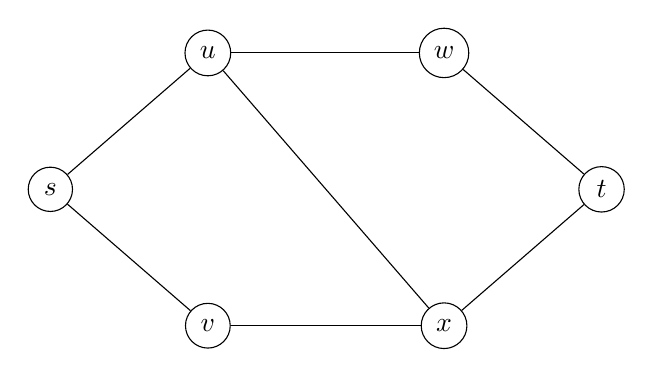
\begin{tikzpicture}[
		wide/.style={line width=4pt},
		every node/.style={circle,draw,minimum size=16},
		scale=2]
		
		\node (s) at (-0.5,0)            {$s$};
		\node (u) at ($ (0,0) + ( 60:1)$) {$u$};
		\node (v) at ($ (0,0) + (-60:1)$) {$v$};
		\node (w) at ($ (u) + ( 1.5,0 )$) {$w$};
		\node (x) at ($ (v) + ( 1.5,0 )$) {$x$};
		\node (t) at ($ (w) + (-60:1) + (0.5,0)$) {$t$};
		
		\draw (s) -- (u);
		\draw (u) -- (w);
		\draw (w) -- (t);
		\draw (s) -- (v);
		\draw (v) -- (x);
		\draw (x) -- (t);
		\draw (u) -- (x);    
		
\end{tikzpicture}
\end{center}

\item \textbf{(b) $[E_T = \{(s, u), (s, v), (u, x), (u, w), (w, t)\}]$} \\
\begin{center}
	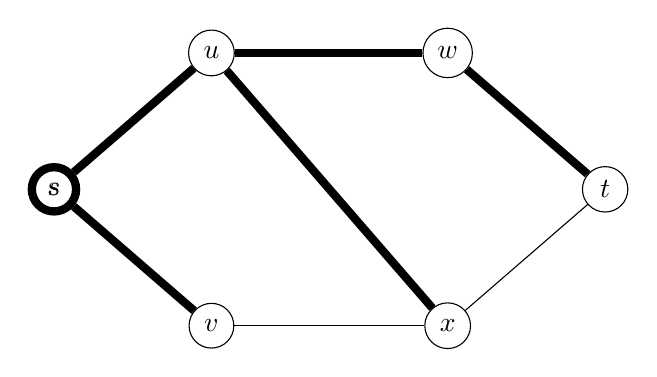
\begin{tikzpicture}[
		wide/.style={line width=4pt},
		every node/.style={circle,draw,minimum size=16},
		scale=2]
		
		\node (s) at (-0.5,0)            {$s$};
		\node (u) at ($ (0,0) + ( 60:1)$) {$u$};
		\node (v) at ($ (0,0) + (-60:1)$) {$v$};
		\node (w) at ($ (u) + ( 1.5,0 )$) {$w$};
		\node (x) at ($ (v) + ( 1.5,0 )$) {$x$};
		\node (t) at ($ (w) + (-60:1) + (0.5,0)$) {$t$};
		
		\draw (s) -- (u);
		\draw (u) -- (w);
		\draw (w) -- (t);
		\draw (s) -- (v);
		\draw (v) -- (x);
		\draw (x) -- (t);
		\draw (u) -- (x);    

		\node[line width=3pt] (s) at (-0.5,0) {s};
		\draw[line width=3pt] (s) -- (v);
		\draw[line width=3pt] (s) -- (u);
		\draw[line width=3pt] (u) -- (x);
		\draw[line width=3pt] (u) -- (w);
		\draw[line width=3pt] (w) -- (t);
		
\end{tikzpicture}
\end{center}

\item \textbf{\\ (c) DFS moves in a penetrating process from one connected node to its next connected node until it reaches the end of its path, thus never resulting in the same tree as per part (b) for any orderings of the vertices, resulting in either $[E_T = \{(s, u), (u, w), (w, t), (t, x), (x, v)\}]$, $[E_T = \{(s, v), (v, x), (x, u), (u, w), (w, t)\}]$, or $[E_T = \{(s, v), (v, x), (x, t), (t, w), (w, u)\}]$. While BFS traverses in a sweeping method before moving deeper to the next level of nodes as highlighted in part (b).} \\
%Your proof goes here.
\end{proof}


%\noindent The following provides a sample of how to draw graphs with \LaTeX. You may use the graph below, or you may come up with your own example.
%\begin{center}
%	\begin{tikzpicture}[
%		wide/.style={line width=4pt},
%		every node/.style={circle,draw,minimum size=16},
%		scale=2]
%		\node (s) at (-0.5,0)            {$s$};
%		\node (u) at ($ (0,0) + ( 60:1)$) {$u$};
%		\node (v) at ($ (0,0) + (-60:1)$) {$v$};
%		\node (w) at ($ (u) + ( 1.5,0 )$) {$w$};
%		\node (x) at ($ (v) + ( 1.5,0 )$) {$x$};
%		\node (t) at ($ (w) + (-60:1) + (0.5,0)$) {$t$};
%		\draw (s) -- (u);
%		\draw (u) -- (w);
%		\draw (w) -- (t);
%		\draw (s) -- (v);
%		\draw (v) -- (x);
%		\draw (x) -- (t);
%		\draw (u) -- (x);    
%		\draw (v) -- (w);

% Replace the line \draw (w) -- (t); with the line below (after deleting the % symbol to uncomment) in order to draw a thicker edge.
%		\node[line width=3pt] (s) at (-0.5,0) {s};
%		\draw[line width=3pt] (s) -- (v);
%		\draw[line width=3pt] (v) -- (x);
%		\draw[line width=3pt] (x) -- (t);
%		\draw[line width=3pt] (t) -- (w);
%		\draw[line width=3pt] (w) -- (u);
		
%\end{tikzpicture}
%\end{center}







\newpage
\subsection{Problem \ref{DFS4}}
\begin{required} \label{DFS4}
	Give an example of a simple, undirected, weighted graph such that a breadth-first traversal outputs a search-tree that is not a single source shortest path tree. (That is, BFS is not sufficiently powerful to solve the shortest-path problem on weighted graphs. This motivates Dijkstra's algorithm, which will be discussed in the near future.) 
	Your answer must
	\begin{enumerate}[label=(\alph*)]
		\item Draw the graph $G = (V,E, w)$ by specifying $V$ and $E$, clearly labeling the edge weights.  [\textbf{Note:} We have provided TikZ code below if you wish to use \LaTeX \ to draw the graph. Alternatively, you may hand-draw $G$ and embed it as an image below, provided that (i) your drawing is legible and (ii) we do not have to rotate our screens to grade your work.]
		\item Specify a spanning tree $T(V, E_{T})$ that is returned by BFS, but is not a single-source shortest path tree. [\textbf{Note:} You may again hand-draw this tree. If you wish, you may clearly mark the edges of $T$ on your drawing of $G$. Please make it easy on the graders to identify the edges of $T$.] 

		\item Specify a valid single-source shortest path tree $T^{\prime} = (V,E_{T^{\prime}})$.  [\textbf{Note:} You may again hand-draw this tree. If you wish, you may clearly mark the edges of $T$ on your drawing of $G$. Please make it easy on the graders to identify the edges of $T$.] 

		\item Include a clear explanation of why the search-tree output by breadth-first search is not a valid single-source shortest path tree of $G$.
	\end{enumerate}
\end{required}


\begin{proof}[Answer:]
\item \textbf{(a) $V = [w, u, x, v, t]$ and $E = [8, 4, 2, 3, 5]$} \\
\begin{center}
	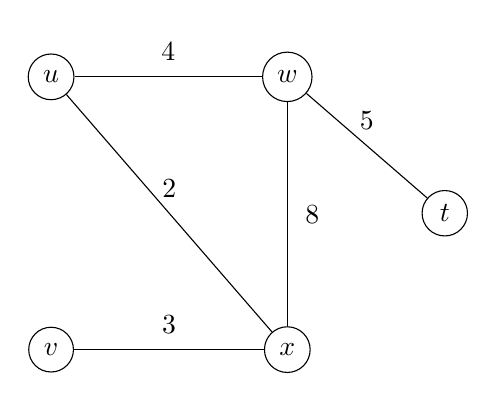
\begin{tikzpicture}[
		wide/.style={line width=4pt},
		every node/.style={circle,draw,minimum size=16},
		scale=2]
		
		\node (u) at ($ (0,0) + ( 60:1)$) {$u$};
		\node (v) at ($ (0,0) + (-60:1)$) {$v$};
		\node (w) at ($ (u) + ( 1.5,0 )$) {$w$};
		\node (x) at ($ (v) + ( 1.5,0 )$) {$x$};
		\node (t) at ($ (w) + (-60:1) + (0.5,0)$) {$t$};

		\draw (u) -- node[above, draw=none,fill=none]{4} (w);
		\draw (w) -- node[above, draw=none,fill=none]{5} (t);		
		\draw (u) -- node[above, draw=none,fill=none]{2} (x);
		\draw (v) -- node[above, draw=none,fill=none]{3} (x);		
		\draw (w) -- node[right, draw=none,fill=none]{8} (x);	
		
\end{tikzpicture}
\end{center}

\item \textbf{(b) BFS spanning tree} \\
\begin{center}
	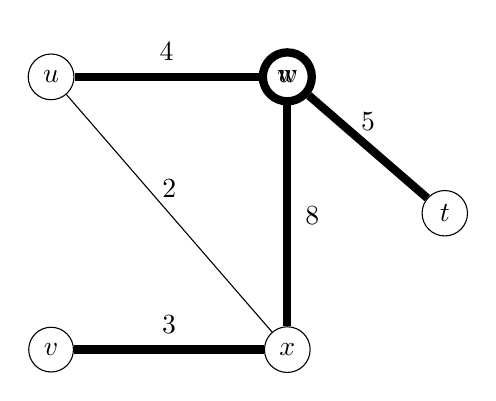
\begin{tikzpicture}[
		wide/.style={line width=4pt},
		every node/.style={circle,draw,minimum size=16},
		scale=2]
		
		\node (u) at ($ (0,0) + ( 60:1)$) {$u$};
		\node (v) at ($ (0,0) + (-60:1)$) {$v$};
		\node (w) at ($ (u) + ( 1.5,0 )$) {$w$};
		\node (x) at ($ (v) + ( 1.5,0 )$) {$x$};
		\node (t) at ($ (w) + (-60:1) + (0.5,0)$) {$t$};

		\node[line width=3pt] (w) at ($ (u) + ( 1.5,0 )$) {w};
		\draw[line width=3pt] (x) -- (v);
		\draw[line width=3pt] (u) -- (w);
		\draw[line width=3pt] (w) -- (x);
		\draw[line width=3pt] (w) -- (t);

		\draw (u) -- node[above, draw=none,fill=none]{4} (w);
		\draw (w) -- node[above, draw=none,fill=none]{5} (t);		
		\draw (u) -- node[above, draw=none,fill=none]{2} (x);
		\draw (v) -- node[above, draw=none,fill=none]{3} (x);		
		\draw (w) -- node[right, draw=none,fill=none]{8} (x);	
		
\end{tikzpicture}
\end{center}

\pagebreak

\item \textbf{(c) Single source shortest path} \\
\begin{center}
	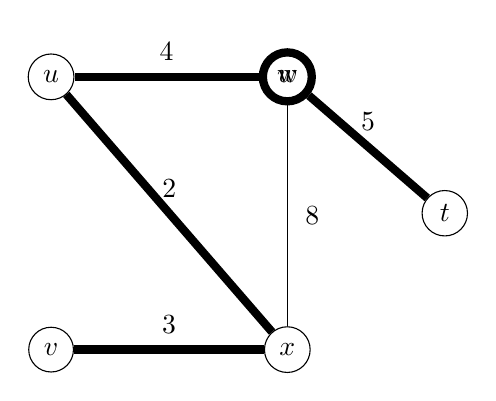
\begin{tikzpicture}[
		wide/.style={line width=4pt},
		every node/.style={circle,draw,minimum size=16},
		scale=2]
		
		\node (u) at ($ (0,0) + ( 60:1)$) {$u$};
		\node (v) at ($ (0,0) + (-60:1)$) {$v$};
		\node (w) at ($ (u) + ( 1.5,0 )$) {$w$};
		\node (x) at ($ (v) + ( 1.5,0 )$) {$x$};
		\node (t) at ($ (w) + (-60:1) + (0.5,0)$) {$t$};

		\node[line width=3pt] (w) at ($ (u) + ( 1.5,0 )$) {w};
		\draw[line width=3pt] (x) -- (v);
		\draw[line width=3pt] (u) -- (w);
		\draw[line width=3pt] (u) -- (x);
		\draw[line width=3pt] (w) -- (t);

		\draw (u) -- node[above, draw=none,fill=none]{4} (w);
		\draw (w) -- node[above, draw=none,fill=none]{5} (t);		
		\draw (u) -- node[above, draw=none,fill=none]{2} (x);
		\draw (v) -- node[above, draw=none,fill=none]{3} (x);		
		\draw (w) -- node[right, draw=none,fill=none]{8} (x);	
		
\end{tikzpicture}
\end{center}

\item \textbf{\\ (d) The algorithm of BFS does not take the weight of the edges into consideration, it only calculates the quantity of edges it traverses. Accordingly, BFS return the spanning tree with the shortest path (i.e. least quantity of edges) from source to goal regardless of the weight of the edges involved. This is notable in the graph of part (b) $[w-x-v]$ which yields a $weight=11$ and $Edges=2$, while the real solution in part (c) $[w-u-x-v]$ yields a $weight=9$ and $Edges=3$. Thus in comparison we can clearly see that BFS does not function as well with the weighted graph in part (a) due to its disregard to weights of the edges.} \\
%Your answer here.
\end{proof}

%\noindent The following provides a sample of how to draw graphs with edge weights using \LaTeX. You may use the graph %below, or you may come up with your own example.
%\begin{center}
%	\begin{tikzpicture}[
%		wide/.style={line width=4pt},
%		every node/.style={circle,draw,minimum size=16},
%		scale=2]
%		\node (s) at (-0.5,0)            {$s$};
%		\node (u) at ($ (0,0) + ( 60:1)$) {$u$};
%		\node (v) at ($ (0,0) + (-60:1)$) {$v$};
%		\node (w) at ($ (u) + ( 1.5,0 )$) {$w$};
%		\node (x) at ($ (v) + ( 1.5,0 )$) {$x$};
%		\node (t) at ($ (w) + (-60:1) + (0.5,0)$) {$t$};


% Replace the line \draw (w) -- (t); with the line below (after deleting the % symbol to uncomment) in order to draw a thicker edge.
%		\draw[line width=3pt] (w) -- (t);


%		\draw (s) -- node[below, draw=none,fill=none]{0} (v);
%		\draw (v) -- node[below, draw=none,fill=none]{0} (x);
%		\draw (x) -- node[below, draw=none,fill=none]{0} (t);
%		\draw (u) edge[bend left=25] node[below, draw=none,fill=none]{0} (x);    
%		\draw (v) edge[bend left=25] node[below, draw=none,fill=none]{0} (w);
%		\draw (s) -- node[above, draw=none,fill=none]{0} (u);
%		\draw (u) -- node[above, draw=none,fill=none]{0} (w);
%		\draw (w) -- node[above, draw=none,fill=none]{0} (t);		
%\end{tikzpicture}
%\end{center}
%%%%%%%%%%%%%%%%%%%%%%%%%%%%%%%%%%%%%%%%%%%%%%%%%%

\end{document} % NOTHING AFTER THIS LINE IS PART OF THE DOCUMENT



